\subsection{Working with multiple EAPs}

Although you can simply copy \& paste single packages between multiple EAPs, packages with dependencies to other packages cannot be copied so easily.
If you do this via copy \& paste all links will be destroyed!

\begin{enumerate}
\item[$\blacktriangleright$] To migrate multiple packages, you have to first export a \emph{complete} root node (a package on the top-most level in the Project
Browser) from the source EAP to XMI. In preparation for a transfer of projects, it might, therefore, make sense to prepare a suitable root node with a relevant
set of projects to be transferred or copied to another (target) EAP file. Right-click the root node you wish to export and select ``Export Model to XMI...''
(Fig.~\ref{fig_projectMigration01}). In the dialogue that pops up, enter the name and path of the exported file and choose \texttt{XMI 2.1} as ``Export type''.

\begin{figure}[htbp]
\begin{center}
  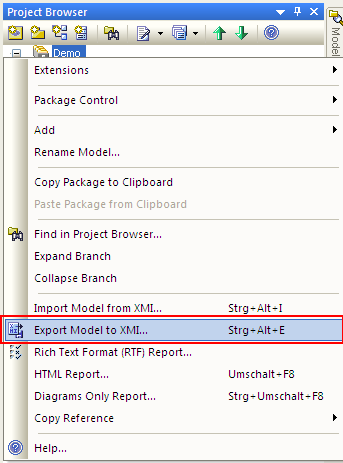
\includegraphics[width=0.5\textwidth]{projectMigration1}
  \caption{Export the root node from the source EAP}
  \label{fig_projectMigration01}
\end{center}
\end{figure}

\item[$\blacktriangleright$] Open the target EAP, right-click on the Project Browser and select ``Import Model from XMI...'' (Fig.~\ref{fig_projectMigration03}).
In the dialogue that pops up, enter the name and path of the file to be imported and click \texttt{Import}.

\begin{figure}[htbp]
\begin{center}
  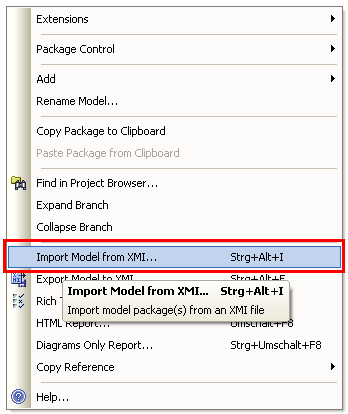
\includegraphics[width=0.5\textwidth]{projectMigration3}
  \caption{Import the root node into the target EAP}
  \label{fig_projectMigration03}
\end{center}
\end{figure}

\item[$\blacktriangleright$] After confirming and starting the import, you have to specify how the model should be imported. As our root models are at the root
level, choose ``Yes'' in the dialogue depicted in Fig.~\ref{fig_projectMigration06}. After the import, you can now delete packages in the root node, which you do not need.

\begin{figure}[htbp]
\begin{center}
  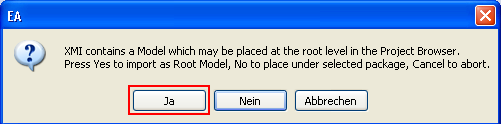
\includegraphics[width=0.5\textwidth]{projectMigration6}
  \caption{Confirm the level of the root node}
  \label{fig_projectMigration06}
\end{center}
\end{figure}

\end{enumerate}
\clearpage
